\documentclass[a4paper]{article}
\usepackage[italian]{babel}
\usepackage[left=1cm, right=1cm, bottom=2cm, top=2cm]{geometry}
\usepackage{csvsimple}
\usepackage[utf8]{inputenc}
\usepackage{float}
\usepackage[table,xcdraw]{xcolor}
\usepackage[scaled]{helvet}
\renewcommand\familydefault{\sfdefault} 
\usepackage{pgfplots}
\pgfplotsset{compat=newest}
\usepackage{multicol}
\usepackage{tabularx}
\usepackage{xcolor}
%opening
\title{Relazione laboratorio Algoritmi Avanzati}
\author{Magarotto Francesco\\Muraro Enrico\\Piva Giulio}

\begin{document}
\rowcolors{2}{gray!25}{white}
\begin{titlepage}
  \vspace*{5cm}
  \begin{center}
    \Large\bfseries
	Relazione di laboratorio
  \end{center}
  \begin{center}
  \large
  Corso di Algoritmi Avanzati\\
  Laurea Magistrale in Informatica\\A.A. 2019-2020
  \end{center}
  \vspace{4cm plus 1fill}
  \begin{flushleft}
  \large
    Magarotto Francesco\\Muraro Enrico\\Piva Giulio
  \end{flushleft}
\end{titlepage}
\newpage

\section{Introduzione}

è valutare le prestazioni dell'algoritmo di Karger per il problema del minimum cut rispetto a quattro parametri:
\begin{itemize}
\item Il tempo impiegato dalla procedura di Full Contraction
\item Il tempo impiegato dall'algoritmo completo per ripetere la contrazione un numero sufficientemente alto di volte
\item Il discovery time, ossia il momento in cui l'algoritmo trova per la prima volta il taglio di costo mimimo
\item L'errore nella soluzione trovata rispetto al risultato ottimo
\end{itemize}
Il linguaggio di programmazione scelto dal nostro gruppo è Java.

\subsection{Esecuzione del programma}
Gli algoritmi sono stati sviluppati come progetto Maven. All'interno della cartella \'e presente la versione portable di Maven, pertanto non è necessario averlo installato. \'E
richiesto almeno il JDK 11 installato nel sistema.
Per eseguire i tre algoritmi utilizzare i seguenti comandi:\\
Linux:\\
\indent \texttt{./mvnw install}\\
\indent \texttt{./mvnw exec:java}\\
Windows:\\
\indent \texttt{mvnw.cmd install}\\
\indent \texttt{mvnw.cmd exec:java}

L'esecuzione del main genera automaticamente dei file csv nella directory del progetto contenenti i tempi registrati. L'algoritmo di Karger viene interrotto dopo 60 secondi.
\subsection{Strutture dati utilizzate}

Per rappresentare il grafo abbiamo utilizzato una matrice di adiacenza visto che i sono grafi completi e la matrice viene quindi riempita senza sprechi di memoria.

Nell'algoritmo 2 Approssimato abbiamo fatto uso di un HashMap per registrare la visita in preordine del grafo.

La classe Heap è una nostra implementazione di MinHeap. L'albero binario è rappresentato da un array di interi, i valori all'interno dell'array corrispondono ai nodi presenti nel grafo. Il confronto tra i nodi per determinare il più piccolo è effettuato tramite un Comparator passato alla creazione dello Heap, questo per avere un'implementazione di Heap indipendente dal modo in cui viene utilizzato da uno specifico algoritmo.
\subsection{Lettura di un grafo da file}
Per caricare un grafo in memoria, abbiamo implementato una classe GraphReader, che si occupa della lettura del file tramite la libreria \textit{nio} di Java. Inoltre effettua le conversioni di distanza necessarie sia per i file di tipo GEO che EUC\_2D e ritorna direttamente la matrice di adiacenza del grafo.


\subsection{Implementazione di Held-Karp}

L'algoritmo di Held-Karp necessita di due strutture di supporto, una per salvare le distanze minime già calcolate e una per ricordare il nodo precedente in modo da poter ricostruire il percoso trovato. Visto che entrambi sono identificati da due valori (v,S) dove 'v' è un nodo e 'S' un insieme di nodi abbiamo deciso di implementare entrambe con ArrayList di HashMap. Ogni posizione dell'ArrayList corrisponde a un nodo e contiene una mappa che ha come chiave un Set di nodi. In questo modo con due accessi costanti possiamo trovare il valore desiderato.

Il timeout di Held-Karp è controllato da un flag booleano, quando viene impostato il valore del flag a 'true' il ciclo che cerca il minimo viene interrotto e l'algoritmo ritorna la soluzione migliore trovata fino a quel momento.

Quando eseguiamo l'algoritmo facciamo quindi partire un thread usando ScheduledExecutorService, che dopo 5 minuti imposta il flag a 'true' terminando l'esecuzione.

\subsection{Implementazione dell'euristica nearest-neighbor}
L'Euristica nearest-neighbor consiste nel trovare il prossimo vertice, non ancora inserito nel circuito, a distanza minima dal nodo corrente. Una volta visitati tutti i nodi
ripetendo questa operazione si otter\'a un percordo 2-approssimato per il problema del TSP. Questa euristica \'e di facile implementazione, ma allo stesso tempo molto efficace.

\subsection{Implementazione dell'algoritmo 2-approssimato}
L'algoritmo 2-approssimato \'e basato su una tecnica molto semplice: Si trova un MST con l'algoritmo di Prim e poi si visita l'albero in ordine prefisso.
Nel nostro caso, Prim restituisce il MST sotto forma di HashMap, dove la chiave \'e un nodo e il value la lista dei suoi figli. A questo punto l'albero viene visitato in ordine
prefisso dal metodo Preorder, restituendo un percorso approssimato per il problema del TSP.

\begin{figure}[H]
\centering
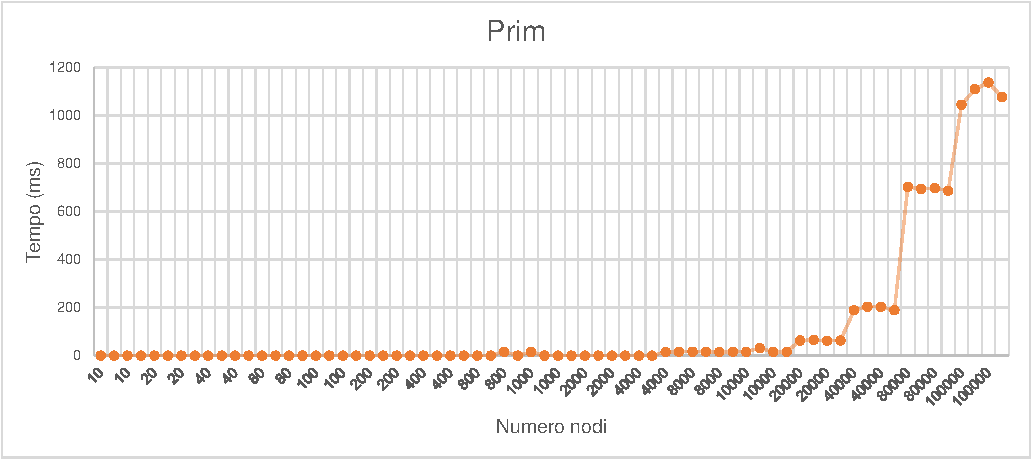
\includegraphics[scale=1]{grafici/prim.pdf}
\caption{Grafico andamento algoritmo di Prim}
\end{figure}

\begin{figure}[H]
\centering
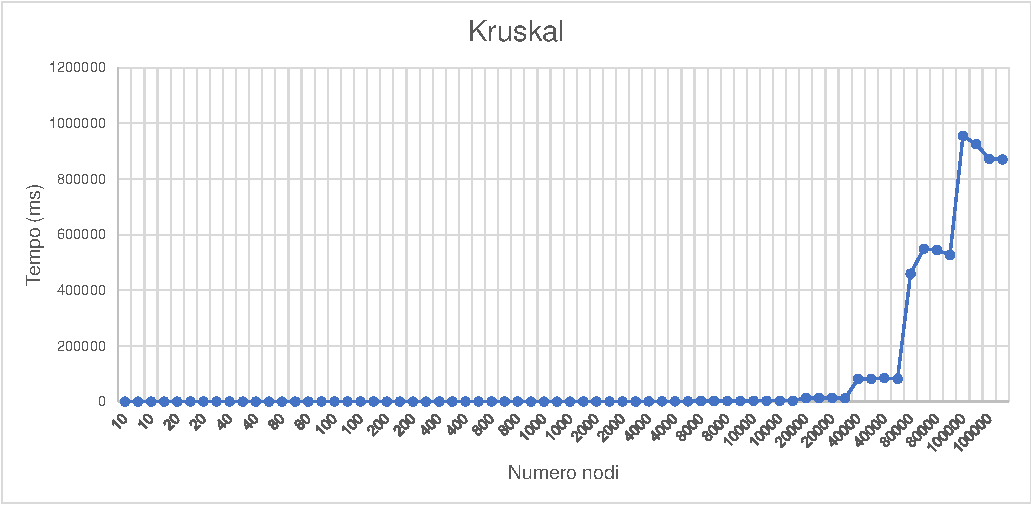
\includegraphics[scale=1]{grafici/kruskal.pdf}
\caption{Grafico andamento algoritmo di Kruskal}
\end{figure}

\begin{figure}[H]
\centering
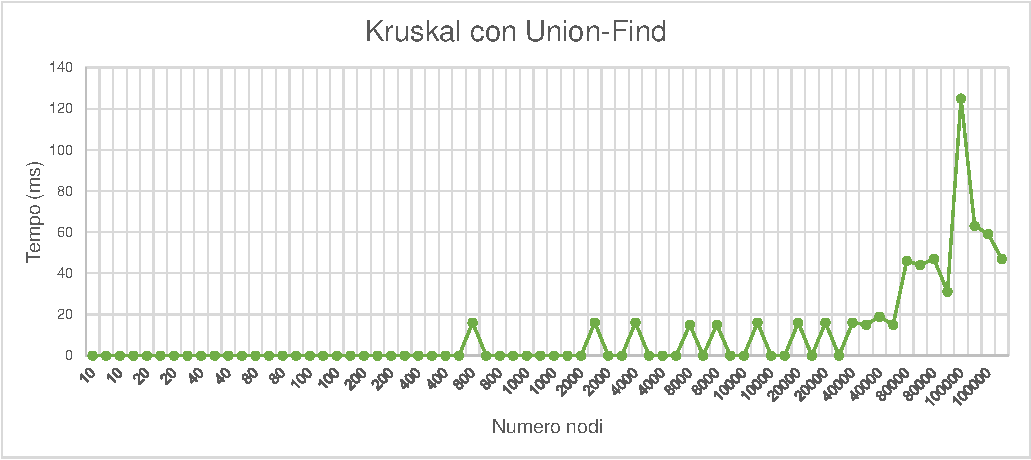
\includegraphics[scale=1]{grafici/kruskaluf.pdf}
\caption{Grafico andamento algoritmo di Kruskal con Union-Find}
\end{figure}

%\begin{figure}[H]
%\centering
%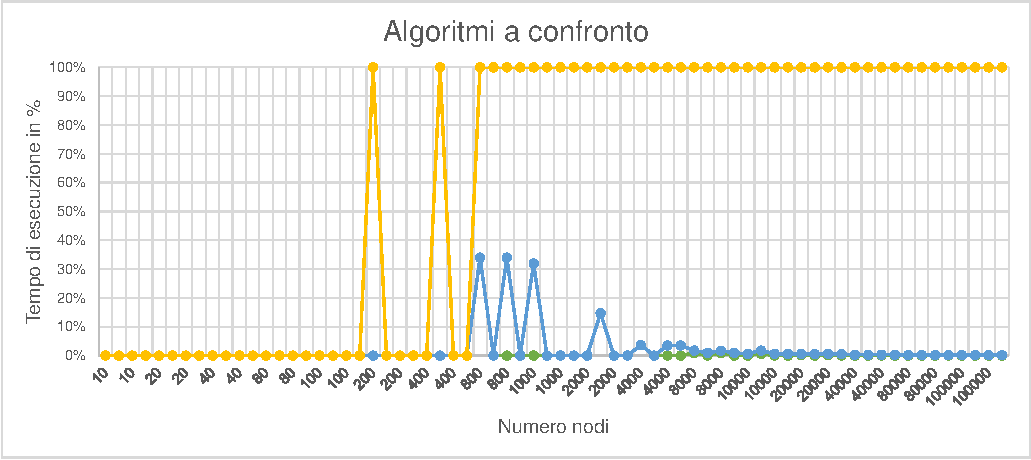
\includegraphics[scale=1]{grafici/confronto.pdf}
%\caption{Grafico che mette in relazione i tempi di esecuzione dei tre algoritmi in base al tempo richiesto per la loro esecuzione}
%\end{figure}

% Please add the following required packages to your document preamble:
% \usepackage[table,xcdraw]{xcolor}
% If you use beamer only pass "xcolor=table" option, i.e. \documentclass[xcolor=table]{beamer}
% Please add the following required packages to your document preamble:
% \usepackage[table,xcdraw]{xcolor}
% If you use beamer only pass "xcolor=table" option, i.e. \documentclass[xcolor=table]{beamer}
\begin{table}[]
\begin{minipage}[b]{10cm}
\begin{tabular}{|c|c|c|c|c|}
\rowcolor{gray!50}
\hline
\textbf{Nodi} & \textbf{Prim} & \textbf{Kruskal UF} & \textbf{Kruskal} & \textbf{MST} \\ \hline
10            & 0              & 0                   & 0                & 29316        \\ \hline
10            & 0              & 0                   & 0                & 2126         \\ \hline
10            & 0              & 0                   & 0                & -44765       \\ \hline
10            & 0              & 0                   & 0                & 20360        \\ \hline
20            & 0              & 0                   & 0                & -32021       \\ \hline
20            & 0              & 0                   & 0                & 18596        \\ \hline
20            & 0              & 0                   & 0                & -42560       \\ \hline
20            & 0              & 0                   & 0                & -37205       \\ \hline
40            & 0              & 0                   & 0                & -122078      \\ \hline
40            & 0              & 0                   & 0                & -37021       \\ \hline
40            & 0              & 0                   & 0                & -79570       \\ \hline
40            & 0              & 0                   & 0                & -79741       \\ \hline
80            & 0              & 0                   & 0                & -139926      \\ \hline
80            & 0              & 0                   & 0                & -211345      \\ \hline
80            & 0              & 0                   & 0                & -110571      \\ \hline
80            & 0              & 0                   & 0                & -233320      \\ \hline
100           & 0              & 0                   & 0                & -141960      \\ \hline
100           & 0              & 0                   & 0                & -271743      \\ \hline
100           & 0              & 0                   & 0                & -288906      \\ \hline
100           & 0              & 0                   & 0                & -232178      \\ \hline
200           & 0              & 0                   & 16               & -510185      \\ \hline
200           & 0              & 0                   & 0                & -515136      \\ \hline
200           & 0              & 0                   & 0                & -444357      \\ \hline
200           & 0              & 0                   & 0                & -393278      \\ \hline
400           & 0              & 0                   & 0                & -1122919     \\ \hline
400           & 0              & 0                   & 31               & -788168      \\ \hline
400           & 0              & 0                   & 0                & -895704      \\ \hline
400           & 0              & 0                   & 0                & -733645      \\ \hline
800           & 0              & 16                  & 31               & -1541291     \\ \hline
800           & 0              & 0                   & 32               & -1578294     \\ \hline
800           & 16             & 0                   & 31               & -1675534     \\ \hline
800           & 0              & 0                   & 15               & -1652119     \\ \hline
1000          & 15             & 0                   & 32               & -2091110     \\ \hline
1000          & 0              & 0                   & 32               & -1934208     \\ \hline
1000          & 0              & 0                   & 31               & -2229428     \\ \hline
1000          & 0              & 0                   & 31               & -2359192     \\ \hline
\end{tabular}
\end{minipage}
\begin{minipage}[b]{10cm}
\begin{tabular}{|c|c|c|c|c|}
\hline
\rowcolor{gray!50}
\textbf{Nodi} & \textbf{Prim} & \textbf{Kruskal UF} & \textbf{Kruskal} & \textbf{MST} \\ \hline
2000          & 0              & 0                   & 109              & -4811598     \\ \hline
2000          & 0              & 16                  & 93               & -4739387     \\ \hline
2000          & 0              & 0                   & 109              & -4717250     \\ \hline
2000          & 0              & 0                   & 125              & -4537267     \\ \hline
4000          & 0              & 16                  & 423              & -8722212     \\ \hline
4000          & 0              & 0                   & 437              & -9314968     \\ \hline
4000          & 15             & 0                   & 412              & -9845767     \\ \hline
4000          & 16             & 0                   & 439              & -8681447     \\ \hline
8000          & 16             & 15                  & 1722             & -17844628    \\ \hline
8000          & 16             & 0                   & 1713             & -18800966    \\ \hline
8000          & 15             & 15                  & 1731             & -18741474    \\ \hline
8000          & 16             & 0                   & 1753             & -18190442    \\ \hline
10000         & 16             & 0                   & 2637             & -22086729    \\ \hline
10000         & 31             & 16                  & 2601             & -22338561    \\ \hline
10000         & 15             & 0                   & 2563             & -22581384    \\ \hline
10000         & 16             & 0                   & 2638             & -22606313    \\ \hline
20000         & 63             & 16                  & 12976            & -45978687    \\ \hline
20000         & 65             & 0                   & 13002            & -45195405    \\ \hline
20000         & 62             & 16                  & 13009            & -47854708    \\ \hline
20000         & 63             & 0                   & 12427            & -46420311    \\ \hline
40000         & 189            & 16                  & 81522            & -92003321    \\ \hline
40000         & 203            & 15                  & 81525            & -94397064    \\ \hline
40000         & 203            & 19                  & 84400            & -88783643    \\ \hline
40000         & 189            & 15                  & 81242            & -93017025    \\ \hline
80000         & 703            & 46                  & 459713           & -186834082   \\ \hline
80000         & 694            & 44                  & 549392           & -185997521   \\ \hline
80000         & 697            & 47                  & 545050           & -182065015   \\ \hline
80000         & 687            & 31                  & 526711           & -180803872   \\ \hline
100000        & 1045           & 125                 & 955113           & -230698391   \\ \hline
100000        & 1110           & 63                  & 925063           & -230168572   \\ \hline
100000        & 1137           & 59                  & 872704           & -231393935   \\ \hline
100000        & 1077           & 47                  & 869876           & -231011693   \\ \hline
\end{tabular}
\end{minipage}
\caption{Tabella dei risultati. Per ogni algoritmo, i valori si riferiscono al tempo di esecuzione, espressi in ms, di quell'algoritmo con un grafo avente $n$ nodi.}
\label{t1}
\end{table}

\newpage
\section{Confronto}
Sicuramente l'algoritmo con costo computazionale più basso è Kruskal con Union-Find.
Confrontiamo quindi l'esecuzione di Kruskal con Union-Find con gli altri due algoritmi partendo da Prim. 
\begin{figure}[H]
\centering
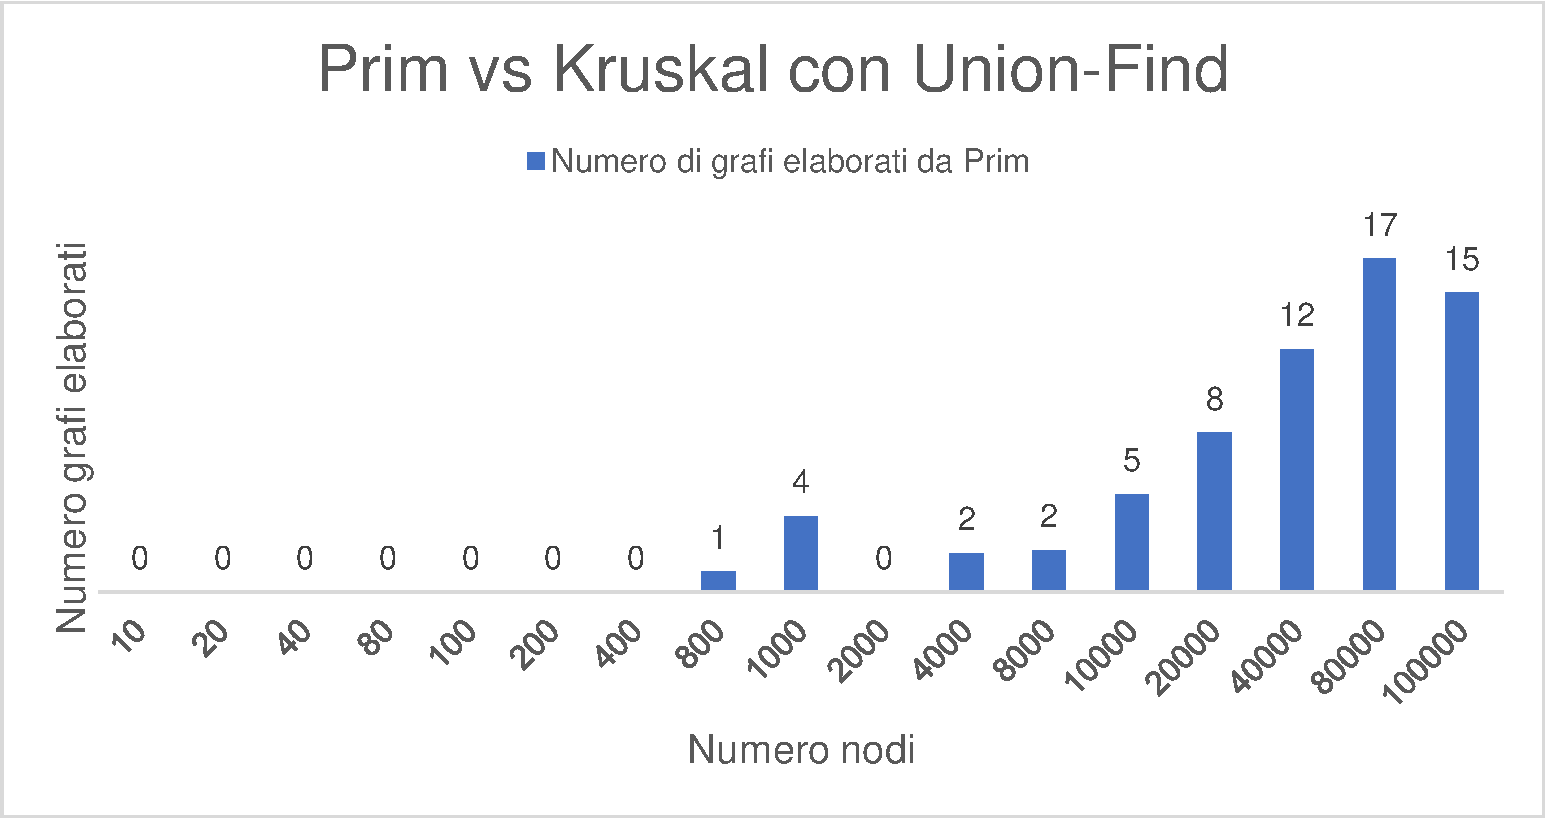
\includegraphics[scale=0.5]{grafici/primvskruskaluf.pdf}
\caption{Numero di grafi di dimensione $n$ che Kruskal con Union-Find è in grado di elaborare nello stesso tempo medio impiegato da Prim per elaborare \textbf{un} grafo  della medesima dimensione. Come possiamo vedere Kruskal con Union-Find è molto più efficiente in grafi di grandi dimensioni. Ad esempio per un grafo di 10\^{}5 nodi, in media, Kruskal con Union-Find è 15 volte più veloce di Prim.
}
\end{figure}
Confrontiamo ora l'algoritmo di Kruskal con Union-Find con la sua versione naive:
\begin{figure}[H]
\centering
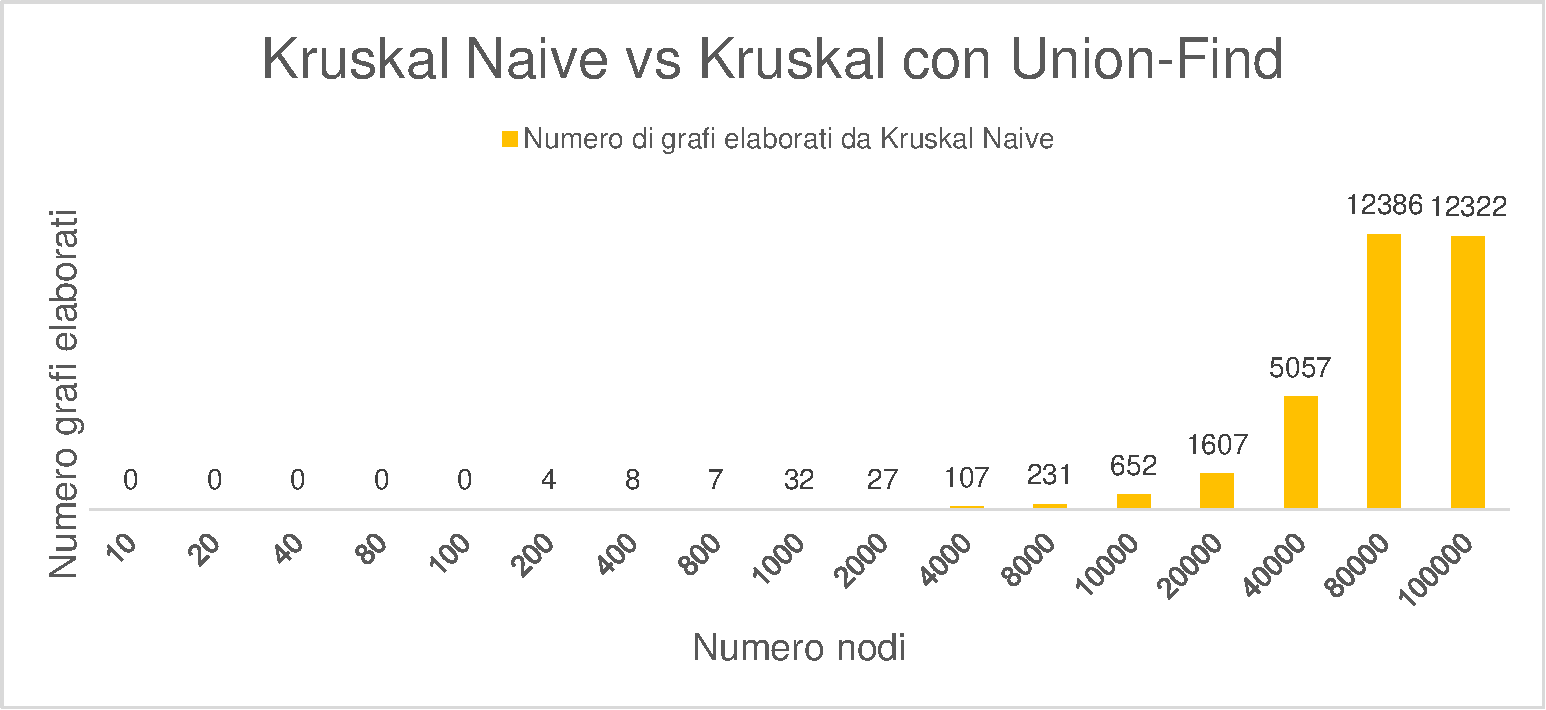
\includegraphics[scale=0.5]{grafici/kruskalvskruskaluf.pdf}
\caption{Numero di grafi di dimensione $n$ che Kruskal con Union-Find è in grado di elaborare nello stesso tempo medio impiegato da Kruskal naive per elaborare \textbf{un} grafo della medesima dimensione. Come possiamo vedere Kruskal è molto più efficiente in grafi di grandi dimensioni. Ad esempio per un grafo di 10\^{}5 nodi, in media, Kruskal con Union-Find è 12322 volte più veloce di Kruskal naive.}
\end{figure}
Da questi due grafici e nella tabella \ref{t1} possiamo affermare che Kruskal con Union-Find è l'algoritmo \textbf{più} efficiente per il calcolo di un MST, segue l'algoritmo di Prim, e infine Kruskal "Naive" che ha il costo computazionale più alto.
\section{Conclusione}
I risultati ottenuti rispecchiano l'andamento che ci aspettavamo conoscendo la complessità degli algoritmi, infatti Kruskal "Naive" di complessità $O(mn)$ ha ottenuto risultati peggiori di qualche ordine di grandezza rispetto agli altri due algoritmi, i quali hanno entrambi complessità $O(m\log{}n)$.

La differenza tra Kruskal con Union-Find e Prim è dovuta probabilmente dalla nostra implementazione degli algoritmi e delle strutture dati che abbiamo utilizzato, ad esempio esistono implementazioni migliori di Prim che utilizzano Heap di Fibonacci per abbassare la complessità a $O(m+n\log{}n)$ e che avrebbero portato a tempi di esecuzione più bassi per i grafi di dimensione maggiore.

In termini di efficienza Kruskal con Union-Find ha ottenuto i tempi di esecuzione più bassi sia per grafi di piccola dimensione sia per i grafi con più di 80000 nodi, ed è quindi l'algoritmo migliore nella nostra implementazione. 

\end{document}
